\documentclass[conference]{IEEEtran}
\hyphenation{op-tical net-works semi-conduc-tor IEEEtran}
\usepackage[bottom=2cm,top=3cm,left=3cm,right=2cm]{geometry}
\usepackage{url}
\makeatletter
\def\ps@pprintTitle{%
	\let\@oddhead\@empty
	\let\@evenhead\@empty
	\def\@oddfoot{\reset@font\hfil\thepage\hfil}
	\let\@evenfoot\@oddfoot
}
\makeatother

\usepackage{babelbib}

\usepackage[brazilian]{babel} % Traduz alguns termos para o português
\usepackage[utf8]{inputenc} % Reconhece acentuação
\usepackage{setspace}
\usepackage{graphicx}


\begin{document}

% paper title
\title{Teoria da Decisão\\ Métodos Escalares de Otimização Vetorial e Tomada de Decisão Assistida}


% author names and affiliations
% use a multiple column layout for up to three different
% affiliations
\author{\IEEEauthorblockN{Rafael Carneiro de Castro}
\IEEEauthorblockA{\\Engenharia de Sistemas - UFMG\\
Matrícula: 2013030210\\
Email: rafaelcarneiroget@hotmail.com}
\and
\IEEEauthorblockN{Davi Pinheiro Viana}
\IEEEauthorblockA{\\Engenharia de Sistemas - UFMG\\
	Matrícula: 2013029912\\
	Email: daviviana22@gmail.com}}

\maketitle

\begin{abstract}
Abordagem de forma conjunta de grande parte dos conceitos vistos na disciplina "ELE088 - Teoria da Decisão", através de um problema de escalonamento de tarefas. O problema foi resolvido através de implementações mono e multiobjetivo e utilizando o método de auxílio à tomada de decisão Programação de Compromissos.
\end{abstract}

\IEEEpeerreviewmaketitle

\section{Introdução}
O presente trabalho tem o objetivo de resolver um problema de otimização, utilizando técnicas escalares de decisão assistida, estudadas em sala de aula, e colocar em prática grande parte dos conceitos da matéria.

O problema a ser resolvido é o seguinte:
\textit{Uma empresa possui um conjunto de M máquinas que devem ser utilizadas para processar N tarefas indivisíveis. Cada máquina $i$ leva um tempo $t_{ij}$ para processar uma tarefa $j$ e pode processar uma única tarefa por vez. Todas as tarefas possuem uma mesma data ideal de entrega $d$, sendo que cada tarefa $j$ sofre uma penalidade $w_j$ proporcional a cada dia que ela é entregue adiantada ou atrasada em relação a $d$.}

Deve ser feita a formulação e resolução do problema nas versões mono e multiobjetivo e também utilização da técnica de análise de decisão \emph{Programação de Compromissos}.

\section{Desenvolvimento}
\subsection{Formulação do Problema:}
A formulação do problema foi dividida em duas partes, como é discutido a seguir:

\subsubsection{Minimização do Tempo Total de Entrega}
Em primeiro momento, é preciso construir uma função objetivo e suas eventuais restrições para minimização do tempo total de entrega de todas as tarefas. Considere $C_i$ como sendo o tempo necessário para se terminar as tarefas executadas pela máquina $i$. Assim:
\[C_i = \sum_{j=1}^{N}t_{ij} \cdot x_{ij}\ \forall\ i \in\ (1,...,M) \]
O objetivo então se torna:
\[\mathrm{min}\ C_{\mathrm{max}} \]
\[C_{\mathrm{max}} = \mathrm{max}(C_i)\ \forall\ i \in\ (1,...,M) \]
sujeito a:

\begin{equation}
	\sum_{i=1}^{N}x_{ij}=1\ \forall\ j \in\ (1,...,M)
	\label{eq:rest1}
\end{equation}
\[ x_{ij} \in (0, 1)\]

A restrição contida na equação \ref{eq:rest1}, garante que todas as tarefas serão cumpridas e, também, que cada tarefa será executada por uma única máquina. A matriz $x$ é composta por zeros e uns. Cada uma das suas linhas, então, vai representar uma tarefa, e cada coluna, uma máquina. O número 1 em uma coluna representa qual máquina vai executar a tarefa daquela linha.

\subsubsection{Minimização da Soma Ponderada dos Atrasos e Adiantamentos}
Agora, uma função objetivo para tratar a minimização da soma ponderada dos atrasos e adiantamentos é formulada. O momento de término da tarefa $j$ será chamado de $e_j$. Então:
\[e_j = \sum{}{}t_{ik}\ \forall\ k \in\ \Omega_j \]
onde $\Omega_j$ é o conjunto das tarefas até a tarefa $j$ executadas por uma mesma máquina $i$. A função objetivo pode ser escrita como:
\[\mathrm{min}\ \sum_{j=1}^{N}w_j|e_j-d| \]
sujeito a:
\begin{equation}
\sum_{i=1}^{M}x_{ij}=1\ \forall\ j \in\ (1,...,N)\\
\label{eq:rest3}
\end{equation}
\[x_{ij} \in (0, 1)\]

onde, como já discutido, $d$ é a data ideal de entrega das tarefas e $w_j$ a penalidade proporcional a cada dia que a tarefa é entregue adiantada ou atrasada em relação a $d$.

A restrição contida na equação \ref{eq:rest3}, garante que todas as tarefas serão cumpridas e, também, que cada tarefa será executada por uma única máquina

\subsection{Algoritmos de Solução:}
Nesta seção serão discutidos e exibidos os algoritmos para solução dos problemas mono e multiobjetivo.
\subsubsection{Minimização do Tempo Total de Entrega}
O algoritmo de otimização utilizado aqui se baseia no \textit{Simulated Annealing}, método estudado em sala de aula de fácil implementação e convergência atrativa. Este método escapa de mínimos locais com a aceitação de alguns movimentos de piora na qualidade da solução. É inspirado no recozimento físico de sólidos, e possui um parâmetro conhecido como \textit{temperatura}, que ajusta a probabilidade de um movimento de piora ser aceito. Um algoritmo simplificado para o \textit{Simulated Annealing} pode ser visto na Figura \ref{fig:algoritmo}.

	\begin{figure}[h]
%		\centering
		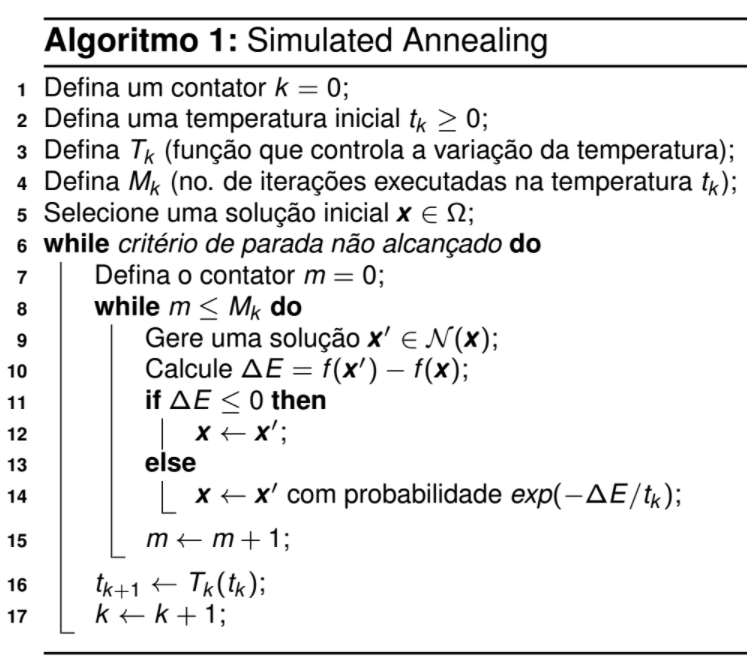
\includegraphics[width=8cm]{img/sa.png}
		\caption{Algoritmo simplificado do SA.}
		\label{fig:algoritmo}
	\end{figure}
	
Para tratar o problema da minimização do tempo de entrega, é importante ter em mente a representação de uma possível solução. Esta representação, como discutido na seção A.1, é uma matriz de zeros e uns, onde o 1 representa qual máquina faz dada tarefa.

A primeira etapa foi criar um algoritmo que gera uma solução inicial. Este código está no arquivo \texttt{initialSolTE.m}. Uma solução é inicializada como sendo uma matriz de zeros. Então, para cada linha (tarefa), um número randômico entre 1 e a quantidade de máquinas é gerado, representado qual é a máquina escolhida para executar a tarefa daquela linha. Um número 1 é colocado na posição da linha do número randômico gerado. Repare que esta solução gerada nunca viola a restrição de que a soma dos valores de uma linha deve ser sempre 1.

Em seguida, criou-se um código que é responsável por avaliar uma dada solução na função objetivo, algoritmo este que está no arquivo \texttt{fobjTE.m}. Este arquivo define a função \emph{fobjTE} que recebe como entrada a solução que se deseja avaliar e uma matriz com o tempo que cada máquina demora para executar cada tarefa (estes tempos são carregados do arquivo \texttt{i5x25.mat} disponibilizado pelo professor). Pela multiplicação vetorial de cada linha da matriz dos tempos com cada coluna da matriz $x$ (solução), tem-se o tempo de operação de cada máquina. A avaliação da solução na função objetivo é, como já visto, o maior dentre os tempos de operação das máquinas.

Antes de implementar o SA propriamente dito, foi necessário também criar funções que geram novas soluções em dada vizinhança. Para este trabalho, duas funções de vizinhança foram criadas. A primeira, para uma dada solução $x$, gera uma nova solução $y$ trocando aleatoriamente as máquinas que executam $n$ tarefas ($n$ também é um parâmetro da função), e está no arquivo \texttt{neighbor1TE.m}. Repare que aqui não ocorre necessariamente uma troca entre máquinas. A outra função de vizinhança recebe uma solução $x$ e gera uma nova solução $y$ escolhendo duas linhas aleatoriamente (duas tarefas), e trocando-as, de forma que duas máquinas trocam as tarefas entre si. Está no arquivo \texttt{neighbor2TE.m}. Com estas funções de vizinhança, a restrição de que cada linha pode ter apenas um número 1 (cada tarefa só pode ser executada por uma máquina) ainda é atendida.

O algoritmo de otimização foi implementado no arquivo \texttt{minTempoEntrega.m}, que tem a função de mesmo nome. Utiliza a estratégia do \textit{Simulated Annealing} e também, como auxílio, todos os outros algoritmos apresentados até aqui para o problema em questão. A função \textit{minTempoEntrega} implementada no arquivo possui dois argumentos, o que vai facilitar, posteriormente, no ajuste de parâmetros do método implementado. Este ajuste será apresentado na seção de resultados.

\subsubsection{Minimização da Soma Ponderada dos Atrasos e Adiantamentos}
TODO
\\
TODO
\\TODO
\subsubsection{Otimização multiobjetivo - Soma ponderada}
Uma versão de resolução do problema apontado anteriormente é a otimização dos dois objetivos ao mesmo tempo (multiobjetivo). Ou seja, ao mesmo tempo em que se minimiza o \emph{tempo total de entrega}, minimiza-se também a \emph{soma ponderada dos atrasos e adiantamentos}. Essa versão do problema é mais próxima da situação real em que sempre se busca os dois objetivos.

O primeiro método  aplicado para resolução da versão mutiobjetivo foi a \emph{Soma Ponderada}. Nele, as duas funções objetivos são agrupadas em uma única função. A nova função objetivo é composta de um somatório ponderado das anteriores e as restrições são as mesmas dos dois problemas. Assim, a função objetivo transformada se torna a seguinte:

\[\mathrm{min}\ p_1 \cdot C_{\mathrm{max}} + p_2 \cdot \left( \sum_{j=1}^{N}w_j|e_j-d| \right)\]
sujeito a:
\begin{equation}
\sum_{i=1}^{M}x_{ij}=1\ \forall\ j \in\ (1,...,N)
\label{eq:rest4}
\end{equation}
\[x_{ij} \in (0, 1)\]
\[p_1 \ge 0\]
\[p_2 \ge 0\]
\[p_1 + p_2 = 1\]

Em que $p_1$ e $p_2$ são os pesos dados às funções objetivos originais.

A função objetivo transformada pode ser resolvida por qualquer método de otimização não linear. No trabalho, foi utilizado um algoritmo também baseado no \emph{Simulated Annealing} (SA), já citado anteriormente. O algoritmo se baseia em um processo que é repetido algumas vezes para encontrar um número finito de soluções Pareto-ótimas, no trabalho foram encontradas 100 (cem) soluções por execução do algoritmo. Esse método foi escolhido por ser simples e fácil de programar e, também, pelo fato da função transformada possuir apenas dois objetivos, já que, para o método da solução ponderada, não são indicadas funções com muitos objetivos pela dificuldade de controlar a diversidade das soluções encontradas. A implementação da resolução do problema pode ser encontrada no arquivo \texttt{SP.m}.

\subsubsection{Otimização multiobjetivo - $\epsilon$-restrito}

O segundo método aplicado para resolução da versão multiobjetivo foi o $\epsilon$-restrito. Nele, escolhe-se uma das funções objetivos para se minimizar e as demais se tornam restrições de desigualdade para o problema transformado. No trabalho, foi escolhido minimizar a função \emph{somatório dos atrasos e adiantamentos} e a função \emph{tempo total de entrega} se tornou uma restrição. Assim, a função objetivo transformada se tornou a seguinte:

\[\mathrm{min}\ \sum_{j=1}^{N}w_j|e_j-d| \]
sujeito a:
\begin{equation}
C_{max} \le \epsilon_1
\end{equation}
\begin{equation}
\sum_{i=1}^{M}x_{ij}=1\ \forall\ j \in\ (1,...,N)\\
\label{eq:rest6}
\end{equation}
\[x_{ij} \in (0, 1)\]

A função objetivo transformada pode ser resolvida por qualquer método de otimização não linear. No trabalho, foi utilizado novamente um algoritmo baseado no \emph{Simulated Annealing} (SA), já citado anteriormente. O algoritmo repete o método SA para encontrar a solução ótima, variando o valor de $\epsilon_1$. O processo é para encontrar um número finito de soluções Pareto-ótimas, no trabalho foram encontradas 100 (cem) soluções por execução do algoritmo. Esse método foi escolhido por ser mais robusto que a \emph{Soma Ponderada} e pelo fato de se ter apenas dois objetivos. O \emph{$\epsilon$-restrito}, para resolução de problemas com mais de dois objetivos, pode gerar funções transformadas infactíveis. A implementação da resolução do problema pode ser encontrada no arquivo \texttt{ER.m}.

\subsection{Resultados:}
Nesta sessão serão apresentados os resultados dos algoritmos.
\subsubsection{Minimização do Tempo Total de Entrega}
Como já mencionado, o algoritmo de otimização foi baseados no \textit{Simulated Annealing}. Esta abordagem exige o ajuste de alguns parâmetros, dentre eles o multiplicador $\alpha$ de temperatura, que é um valor entre $0$ e $1$, que vai diminuir gradualmente a temperatura do algoritmo, e consequentemente diminuir a probabilidade de se aceitar um movimento de piora na busca pela melhor solução. Outro parâmetro que deve ser ajustado é a quantidade $n$ de tarefas que terão a máquina aleatoriamente trocada, na primeira função de vizinhança. Os dados para execução do problema foram disponibilizados pelo professor, são carregados pelo arquivo \texttt{i5x25.mat} e podem ser vistos na tabela da Figura \ref{fig:tabela-dados}.

	\begin{figure}[h]
		\centering
		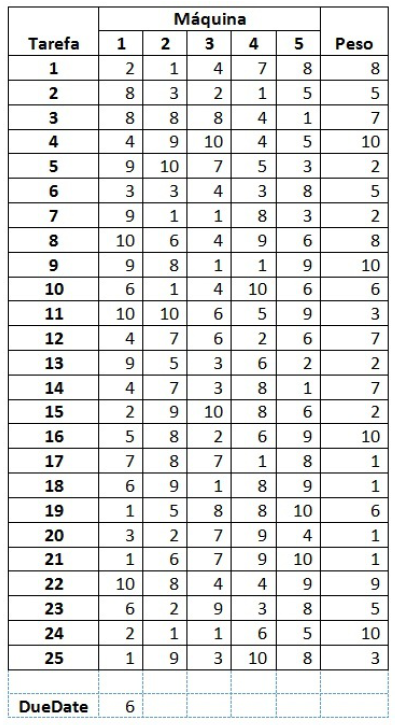
\includegraphics[width=5cm]{img/tabela-dados.png}
		\caption{Tabela de dados para execução dos algoritmos.}
		\label{fig:tabela-dados}
	\end{figure}

Para demonstrar os efeitos da temperatura (parâmetro $\alpha$), uma primeira instancia foi executada, utilizando como parâmetros $\alpha = 0.5$ e $n = 3$. A Figura \ref{fig:result-1} mostra um primeiro resultado desta execução, plotando a avaliação da solução aceita por cada iteração. Como se pode notar, no início do algoritmo, muitas soluções de piora são aceitas, e aos poucos são aceitos cada vez mais apenas movimentos de melhora. Esta execução passou por 2141 iterações e a melhor solução encontrada possui avaliação na função objetivo igual a 20.

	\begin{figure}[h]
		\centering
		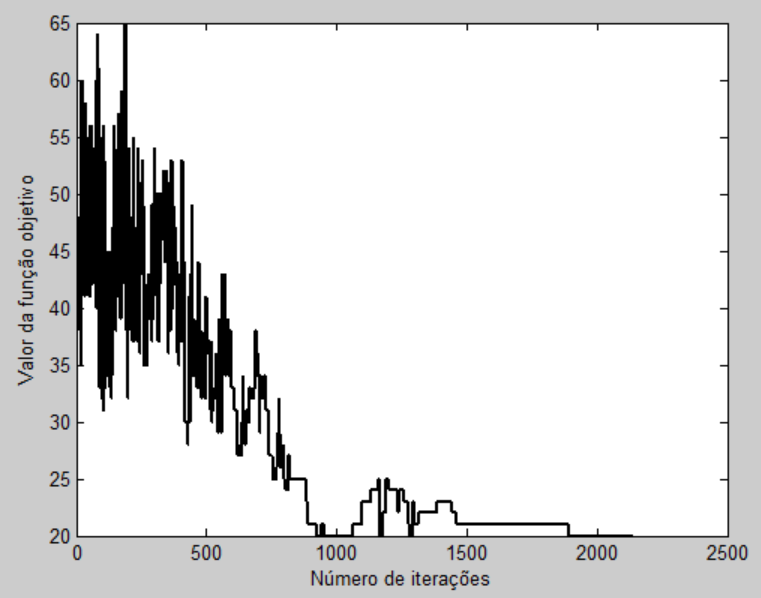
\includegraphics[width=8cm]{img/result-1.png}
		\caption{Primeiro resultado para execução com $\alpha = 0.5$ e $n = 3$.}
		\label{fig:result-1}
	\end{figure}

Executando mais uma vez, mas agora para $\alpha = 0.1$ e $n = 3$, obtemos o resultado mostrado na Figura \ref{fig:result-2}. Como se pode notar, agora menos movimentos de piora são aceitos nas iterações iniciais. Neste caso foram executadas 2488 iterações, com um valor ótimo igual a 14. Ao custo de mais iterações, obteve-se uma ponto de ótimo local melhor.

	\begin{figure}[h]
		\centering
		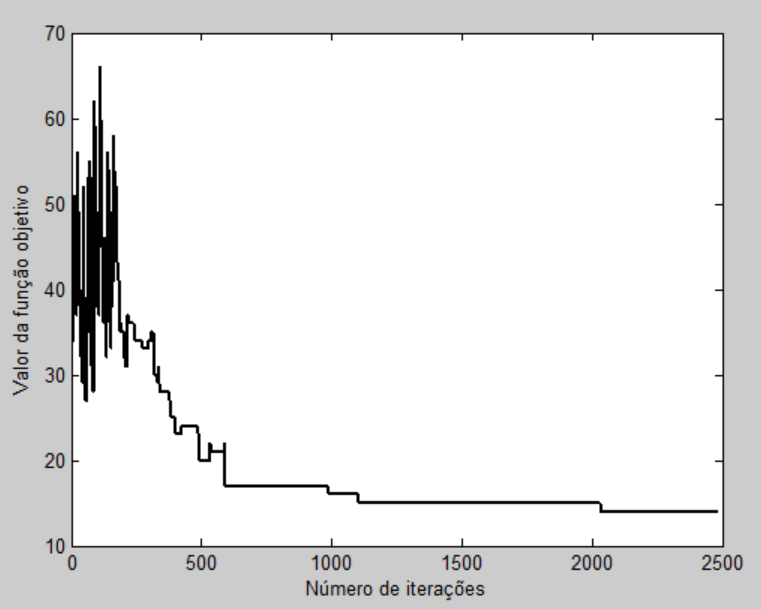
\includegraphics[width=8cm]{img/result-2.png}
		\caption{Primeiro resultado para execução com $\alpha = 0.1$ e $n = 3$.}
		\label{fig:result-2}
	\end{figure}

É necessário então escolher quais serão os parâmetros utilizados, e ainda qual será a função de vizinhança usada. Para tanto, um script de execução foi criado e está no arquivo \texttt{multirunTE.m}. Neste, o código é executado uma quantidade de vezes desejada, e os valores de ótimo e quantidade de iterações para cada execução são plotados. Ajustando o algoritmo para $\alpha = 0.5$ e $n = 3$, após 100 execuções obtemos o resultado mostrado na Figura \ref{fig:mult-result-1}. A linha preta no meio dos gráficos representa a média dos valores. Encontrou-se valor ótimo médio igual a $17,83$ e valor médio da quantidade de iterações igual a $2209,1$.

	\begin{figure}[h]
		\centering
		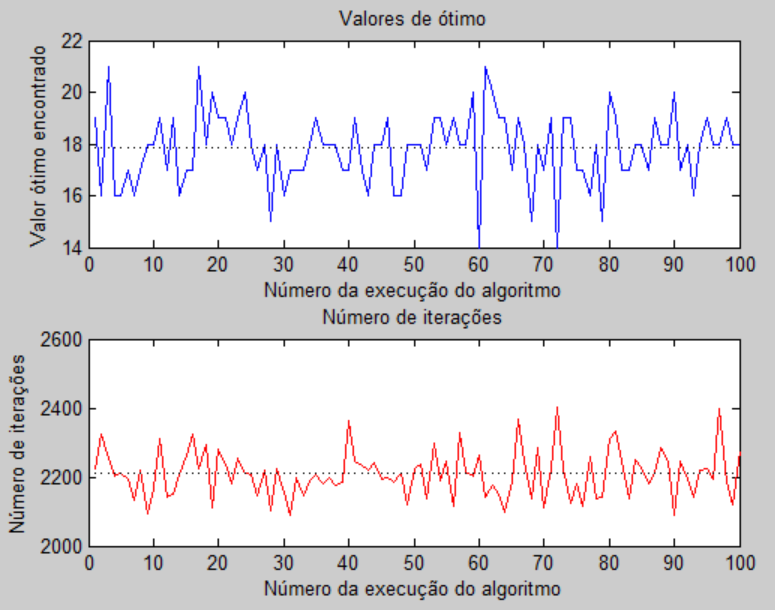
\includegraphics[width=8cm]{img/mult-result-1.png}
		\caption{100 execuções com $\alpha = 0.5$ e $n = 3$.}
		\label{fig:mult-result-1}
	\end{figure}

Foi experimentado também a execução do algoritmo com $\alpha = 0.1$ e $\alpha = 0.01$, ambos mantendo $n = 3$. Os resultados podem ser vistos nas Figuras \ref{fig:mult-result-2} e \ref{fig:mult-result-3}, respectivamente. Para o primeiro caso, a média do valor ótimo foi $14,87$ (com mínimo em $12$ e máximo em $21$) e a média da quantidade de iterações foi $2253,6$ (com mínimo em $2001$ e máximo em $2623$). Para o segundo caso, a média do valor ótimo foi $15,95$ (com mínimo em $13$ e máximo em $19$) e a média da quantidade de iterações foi $2509,4$ (com mínimo em $2299$ e máximo em $2581$). Optou-se então por manter o algoritmo ajustado a $\alpha = 0.1$, por ter uma média de valor ótimo alcançado melhor.

	\begin{figure}[h]
		\centering
		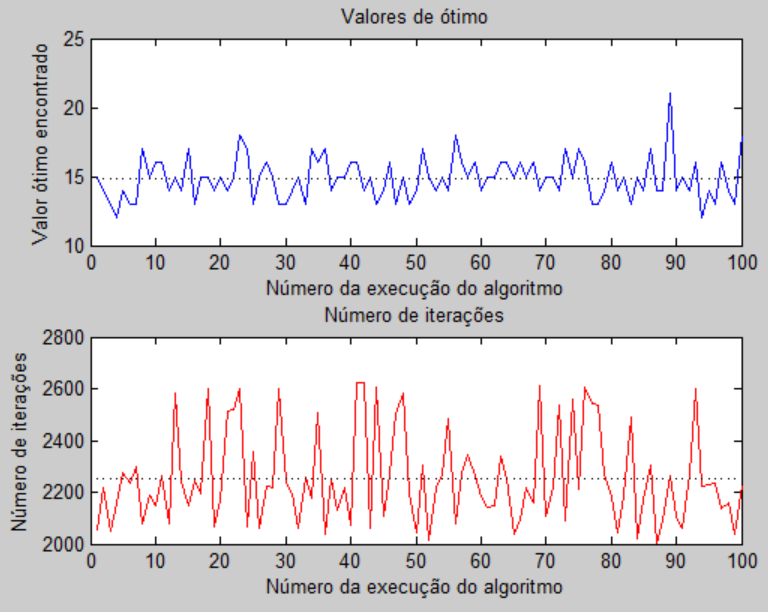
\includegraphics[width=8cm]{img/mult-result-2.png}
		\caption{100 execuções com $\alpha = 0.1$ e $n = 3$.}
		\label{fig:mult-result-2}
	\end{figure}
	
	\begin{figure}[h]
		\centering
		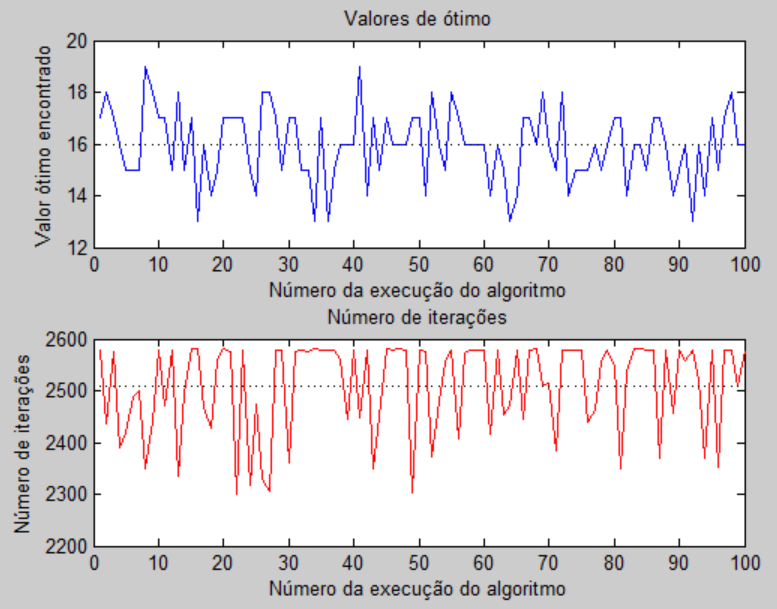
\includegraphics[width=8cm]{img/mult-result-3.png}
		\caption{100 execuções com $\alpha = 0.01$ e $n = 3$.}
		\label{fig:mult-result-3}
	\end{figure}
	
Como todos estes resultados foram obtidos executando o algoritmo com a primeira forma de vizinhança (\textit{neighbor1TE}), precisamos também decidir um valor para $n$. Mantendo $\alpha = 0.1$, \texttt{multirunTE.m} foi executado para $n = 5$ e $n = 1$. Os resultados podem ser vistos nas Figuras \ref{fig:mult-result-4} e \ref{fig:mult-result-5}, respectivamente. Para o primeiro caso, a média do valor ótimo foi $18,29$ (com mínimo em $15$ e máximo em $22$) e a média da quantidade de iterações foi $2059$ (com mínimo em $2044$ e máximo em $2085$). Para o segundo caso, a média do valor ótimo foi $14,77$ (com mínimo em $12$ e máximo em $20$) e a média da quantidade de iterações foi $2260,8$ (com mínimo em $2003$ e máximo em $2622$). Escolhemos então manter $n = 1$.

	\begin{figure}[h]
		\centering
		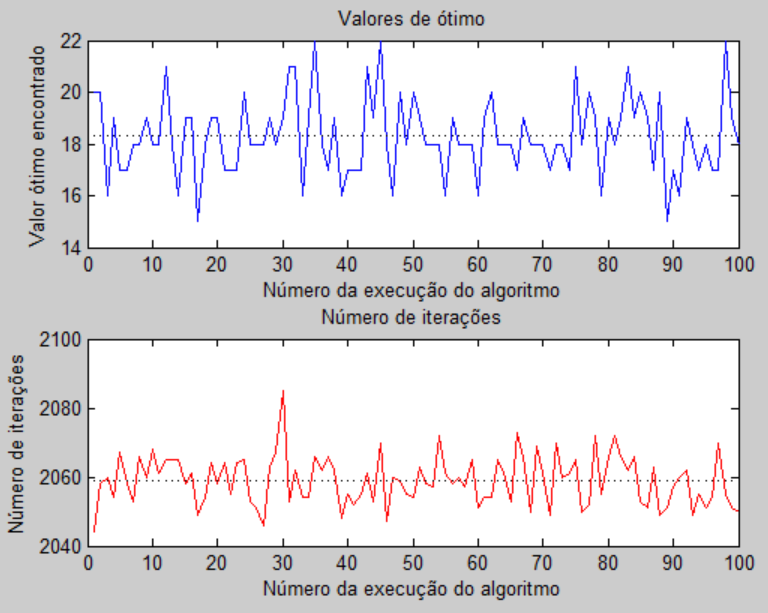
\includegraphics[width=8cm]{img/mult-result-4.png}
		\caption{100 execuções com $\alpha = 0.1$ e $n = 5$.}
		\label{fig:mult-result-4}
	\end{figure}
	
	\begin{figure}[h]
		\centering
		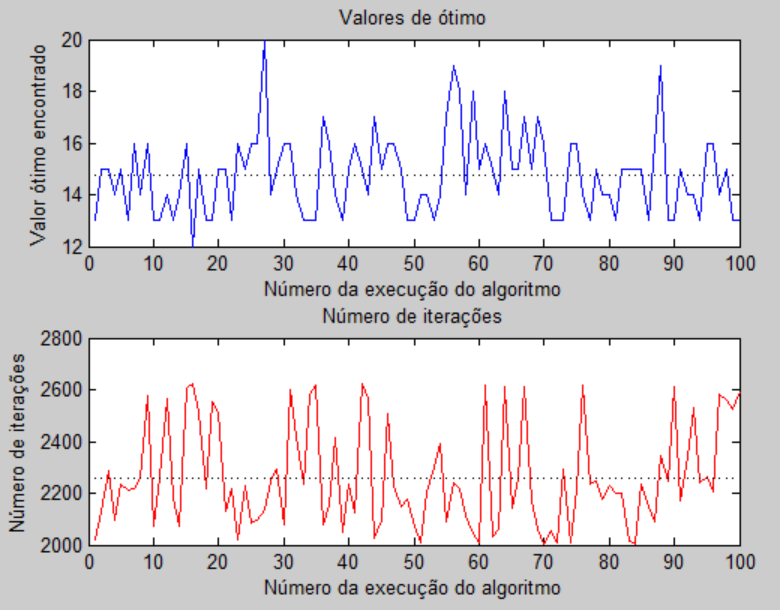
\includegraphics[width=8cm]{img/mult-result-5.png}
		\caption{100 execuções com $\alpha = 0.1$ e $n = 1$.}
		\label{fig:mult-result-5}
	\end{figure}
	
Todos os resultados vistos até aqui foram com o algoritmo rodando apenas com a função de vizinhança \textit{neighbor1TE}. Agora será incorporado ao algoritmo a função \textit{neighbor2TE} seguidamente à primeira, de forma que os dois processos de vizinhança serão executados, um seguido do outro, para se alcançar maior região de busca. Com o auxilio do \texttt{multirunTE.m}, o código foi mais uma vez executado 100 vezes com $\alpha = 0.1$ e $n = 1$, e os resultados podem ser vistos na Figura \ref{fig:mult-result-6}. A média do valor ótimo foi $14,12$ (com mínimo em $12$ e máximo em $16$) e a média da quantidade de iterações foi $2356,5$ (com mínimo em $2043$ e máximo em $2568$). O desempenho foi perceptivelmente melhorado, já que uma maior região de busca é considerada, e melhores ótimos locais são alcançados.

	\begin{figure}[h]
		\centering
		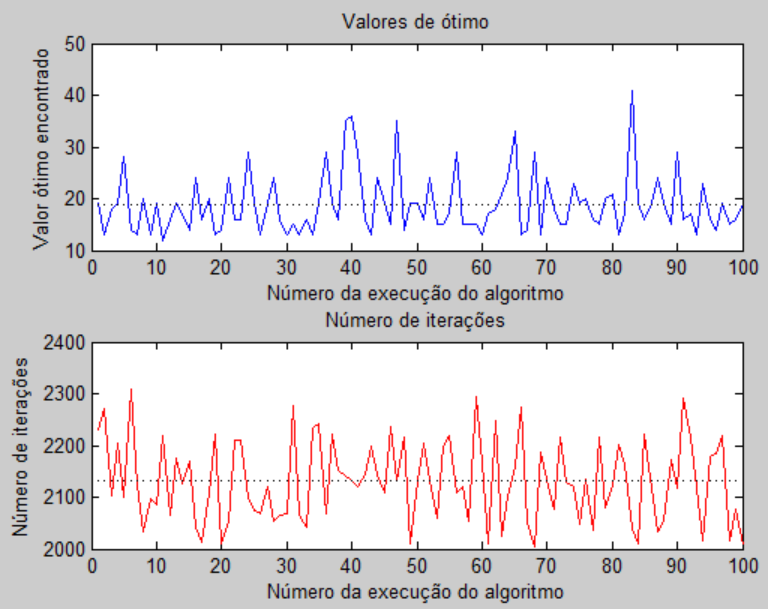
\includegraphics[width=8cm]{img/mult-result-6.png}
		\caption{100 execuções com $\alpha = 0.1$, $n = 1$ e vizinhança \textit{neighbor2TE} adicionada ao código.}
		\label{fig:mult-result-6}
	\end{figure}
	
Com todos os ajustes feitos, o algoritmo foi executado mais 5 vezes, e o resultado sumarizado pode ser visto na Figura \ref{fig:mult-result-7}. Os resultados numéricos são apresentados na Tabela 1.

	\begin{figure}[h]
		\centering
		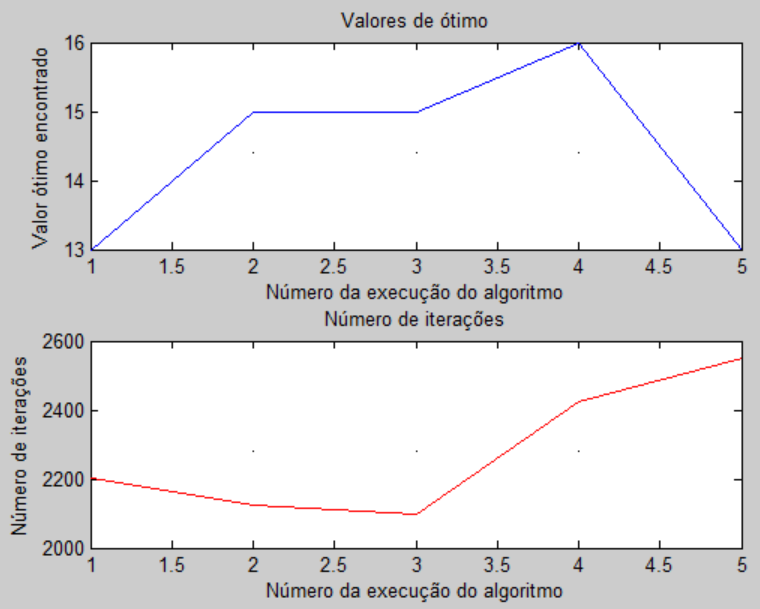
\includegraphics[width=8cm]{img/mult-result-7.png}
		\caption{Resultado final para 5 iterações - Minimização do Tempo de Entrega.}
		\label{fig:mult-result-7}
	\end{figure}
	
	\begin{table}
		\centering
		\begin{tabular}{ | l | l | l | l |}
			\hline
			Ótimo Encontrado & Iterações \\ \hline
			15 & 2336 \\ \hline
			14 & 2440 \\ \hline
			13 & 2392 \\ \hline
			15 & 2228 \\ \hline
			12 & 2330 \\ \hline
		\end{tabular}
		\label{table:result}
		\caption{Resultados numéricos - Minimização do Tempo de Entrega.}
	\end{table}
% Reminder: the "draftcls" or "draftclsnofoot", not "draft", class option
% should be used if it is desired that the figures are to be displayed while
% in draft mode.

% An example of a floating figure using the graphicx package.
% Note that \label must occur AFTER (or within) \caption.
% For figures, \caption should occur after the \includegraphics.
%
%\begin{figure}
%\centering
%\includegraphics[width=2.5in]{myfigure}
% where an .eps filename suffix will be assumed under latex, 
% and a .pdf suffix will be assumed for pdflatex
%\caption{Simulation Results}
%\label{fig_sim}
%\end{figure}


% An example of a double column floating figure using two subfigures.
%(The subfigure.sty package must be loaded for this to work.)
% The subfigure \label commands are set within each subfigure command, the
% \label for the overall fgure must come after \caption.
% \hfil must be used as a separator to get equal spacing
%
%\begin{figure*}
%\centerline{\subfigure[Case I]{\includegraphics[width=2.5in]{subfigcase1}
% where an .eps filename suffix will be assumed under latex, 
% and a .pdf suffix will be assumed for pdflatex
%\label{fig_first_case}}
%\hfil
%\subfigure[Case II]{\includegraphics[width=2.5in]{subfigcase2}
% where an .eps filename suffix will be assumed under latex, 
% and a .pdf suffix will be assumed for pdflatex
%\label{fig_second_case}}}
%\caption{Simulation results}
%\label{fig_sim}
%\end{figure*}



% An example of a floating table. Note that, for IEEE style tables, the 
% \caption command should come BEFORE the table. Table text will default to
% \footnotesize as IEEE normally uses this smaller font for tables.
% The \label must come after \caption as always.
%
%\begin{table}
%% increase table row spacing, adjust to taste
%\renewcommand{\arraystretch}{1.3}
%\caption{An Example of a Table}
%\label{table_example}
%\begin{center}
%% Some packages, such as MDW tools, offer better commands for making tables
%% than the plain LaTeX2e tabular which is used here.
%\begin{tabular}{|c||c|}
%\hline
%One & Two\\
%\hline
%Three & Four\\
%\hline
%\end{tabular}
%\end{center}
%\end{table}


\section{Conclusão}
LEMBRAR DE FALAR QUE O SA É BOM PARA OBTER BONS \textit{ÓTIMOS LOCAIS}, NÃO NECESSARIAMENTE ENCONTRANDO O ÓTIMO GLOBAL.

% conference papers do not normally have an appendix

% use section* for acknowledgement
\section*{Acknowledgment}
% optional entry into table of contents (if used)
%\addcontentsline{toc}{section}{Acknowledgment}
The authors would like to thank...

% trigger a \newpage just before the given reference
% number - used to balance the columns on the last page
% adjust value as needed - may need to be readjusted if
% the document is modified later
%\IEEEtriggeratref{8}
% The "triggered" command can be changed if desired:
%\IEEEtriggercmd{\enlargethispage{-5in}}

% references section
% NOTE: BibTeX documentation can be easily obtained at:
% http://www.ctan.org/tex-archive/biblio/bibtex/contrib/doc/

% can use a bibliography generated by BibTeX as a .bbl file
% standard IEEE bibliography style from:
% http://www.ctan.org/tex-archive/macros/latex/contrib/supported/IEEEtran/bibtex
%\bibliographystyle{IEEEtran.bst}
% argument is your BibTeX string definitions and bibliography database(s)
%\bibliography{IEEEabrv,../bib/paper}
%
% <OR> manually copy in the resultant .bbl file
% set second argument of \begin to the number of references
% (used to reserve space for the reference number labels box)
\begin{thebibliography}{1}

\bibitem{IEEEhowto:kopka}
H.~Kopka and P.~W. Daly, \emph{A Guide to {\LaTeX}}, 3rd~ed.\hskip 1em plus
  0.5em minus 0.4em\relax Harlow, England: Addison-Wesley, 1999.

\end{thebibliography}


% that's all folks
\end{document}


